\documentclass[11pt]{article}

% --- packages (all standard in a full TeX Live / MacTeX install) ---
\usepackage[utf8]{inputenc}
\usepackage[T1]{fontenc}
\usepackage{lmodern}
\usepackage[margin=1in]{geometry}
\usepackage{graphicx}
\usepackage{amsmath,amssymb}
\usepackage{booktabs}
\usepackage{caption}
\usepackage{subcaption}
\usepackage{float}
\usepackage{xcolor}
\usepackage[colorlinks=true,linkcolor=blue,citecolor=blue,urlcolor=blue]{hyperref}
\usepackage{microtype}

\captionsetup{font=small,labelfont=bf}
\newcommand{\lhat}{\hat{\lambda}}

% NOTE TO AUTHORS: fill in the real author/affiliation list and verify the
% references in the bibliography (marked indicative) before submitting.
\title{\textbf{A Local--Geometry Changepoint Aligned with the Onset of\\
Portuguese Grammatical Competence in a Small Language Model}}
\author{Elvis Sikora \quad\textit{[co-author TBA]}\\[2pt]
\small Apart Research Sprint --- June 2026}
\date{\today}

\begin{document}
\maketitle

\begin{abstract}
\noindent
We ask whether a quantity from singular learning theory (SLT) --- the
\emph{local learning coefficient} (LLC, $\lhat$), estimated by stochastic-gradient
Langevin dynamics (SGLD) --- changes in a way that is \emph{aligned with a
behavioral developmental transition} as a small English-trained language model
acquires a second language. We adapt \texttt{TinyStories-8M} to Portuguese by
full-parameter continued pretraining and track, at every checkpoint, both
behavior (validation bits-per-byte and a 538-item grammatical minimal-pair
benchmark) and the LLC. The model's modeling loss falls smoothly, but
grammatical competence emerges \emph{abruptly} (minimal-pair accuracy
chance~$\rightarrow$~$89\%$, with the preference margin flipping sign at
$\approx\!2.5$M tokens). Over exactly this window the LLC \emph{rises steeply}
($+52\rightarrow+87$) and then plateaus --- an aligned-changepoint signature.
Two controls confirm specificity: a token-shuffled-Portuguese model (no word
order to learn) and a matched-English model (generic adaptation) \emph{do not}
reproduce the rise-then-plateau, and the structured model is cleanly separated
from both at $100$M tokens ($+87$ vs.\ $+28$ vs.\ $+70$). The trajectory shape is
robust to the SGLD localization strength. We frame this, following standard
caution, as a changepoint in an SLT-derived local geometric estimate aligned
with a behavioral transition --- not a formal phase transition --- and we are
explicit about the present single-seed scope (a second-seed replication is in
progress).
\end{abstract}

\section{Introduction}
Developmental interpretability asks whether internal, structural quantities of a
neural network change at the moments its behavior changes. Singular learning
theory provides one such quantity: the \emph{local learning coefficient}
(LLC, also called the local RLCT), a measure of the effective dimensionality /
degeneracy of the loss landscape around a parameter
\cite{watanabe2009,lau2024}. If the geometry reorganizes precisely as a
capability appears, the LLC should exhibit a changepoint aligned with the
behavioral one.

We study this in a deliberately small, controllable setting: second-language
acquisition by continued pretraining. We take an English-trained model
(\texttt{TinyStories-8M}) and adapt it to Portuguese, measuring behavior and the
LLC along the whole trajectory. \textbf{The model learning Portuguese is not the
result --- it is the scaffolding.} The contribution is the
\emph{LLC$\leftrightarrow$behavior alignment}, established together with the
controls that make it specific. Our findings:
\begin{itemize}\itemsep2pt
  \item Behavior shows a clean grammatical transition at $\approx\!1.5$--$2.5$M
  tokens even though bits-per-byte falls smoothly (Section~\ref{sec:behavior}).
  \item The LLC rises steeply through that window and then plateaus --- a
  changepoint aligned with the behavioral one (Section~\ref{sec:llc}).
  \item Two controls (shuffled-PT, matched-English) fail to reproduce the
  signature, so it is specific to genuine language structure being acquired,
  not to training length or generic adaptation (Section~\ref{sec:controls}).
  \item The trajectory shape is robust to the SGLD localization hyperparameter
  (Section~\ref{sec:robust}).
\end{itemize}

\section{Setup}\label{sec:setup}
\paragraph{Model and training.} We adapt \texttt{roneneldan/TinyStories-8M} by
full-parameter, FP32 next-token continued pretraining (AdamW, learning rate
$10^{-4}$, $3\%$ warmup, cosine decay, gradient clipping $1.0$, weight decay
$0.01$, batch size $64$, sequence length $128$) on a Portuguese Wikipedia
corpus, to $100$M tokens, with $17$ log-spaced checkpoints. The recipe was fixed
by a short ``autoresearch'' search after an initial under-trained run; we then
froze it across all conditions.

\paragraph{Conditions.} Following the minimal design for this question we run
(i) \emph{structured Portuguese} (the condition of interest), and two controls:
(ii) \emph{token-shuffled Portuguese} --- the same tokens with within-sequence
order destroyed, so there is no grammar to acquire --- and (iii)
\emph{matched English} --- the identical protocol on English, controlling for
``any continued pretraining raises complexity.''

\paragraph{Behavioral metrics (every checkpoint).} Portuguese validation
bits-per-byte (BPB), English-retention BPB, and a frozen, hashed \textbf{538-item
templated Portuguese grammatical minimal-pair benchmark} (10 agreement
phenomena). Accuracy is the fraction of pairs for which the model assigns higher
log-probability to the grammatical sentence; we also report the mean log-prob
margin.

\paragraph{LLC estimation.} We estimate the LLC by SGLD
\cite{lau2024,hoogland2024} using the \texttt{devinterp} library, with one
globally fixed sampler configuration across each trajectory (3 chains, learning
rate $10^{-5}$, $n_\beta\!=\!10$, localization $100$, batch $64$, $200$ burn-in $+$
$100$ draws). With $L$ the loss and $L_0$ the loss at the checkpoint center,
\begin{equation}
  \lhat \;=\; n_\beta \,\big(\mathbb{E}_{\text{SGLD}}[L] - L_0\big),
\end{equation}
which is positive at a true local minimum of the measured loss. \textbf{Crucially,
each condition is measured against a reference set drawn from \emph{its own}
training distribution} (full-length, non-padded chunks): $\lhat$ is only valid at
a minimum of the loss the model actually minimized, so using one condition's data
to score another would yield meaningless estimates.

\paragraph{A measurement note (why the controls matter twice).} An early version
of our LLC pipeline built its reference from short sentences padded to the
sequence length without masking, so $\approx\!90\%$ of every scored sequence was
unmasked padding. This produced \emph{negative} $\lhat$ everywhere --- the
checkpoint is not a minimum of \emph{that} (padded) loss. The fix was to score
non-padded chunks of the actual training distribution. We flag this because it is
the central methodological lesson: an LLC estimate is only meaningful relative to
a loss the model truly minimized, and one must read the \emph{value, sign and
chain agreement}, never a binary ``accepted'' label.

\section{Results}

\subsection{Behavior: smooth loss, abrupt grammar}\label{sec:behavior}
The model genuinely acquires Portuguese: PT BPB falls monotonically
$6.69\rightarrow2.54$ with no kink (Figure~\ref{fig:behavior}). Grammatical
competence, by contrast, emerges abruptly: minimal-pair accuracy sits at chance
through $1.5$M tokens, the mean margin flips negative$\rightarrow$positive
between $1.5$M and $2.5$M, and accuracy then climbs to $89.2\%$ by $27$M
(Table~\ref{tab:behavior}). The abruptness lives in the discrete grammatical
behavior, not in the modeling-loss curve.

\begin{figure}[H]
  \centering
  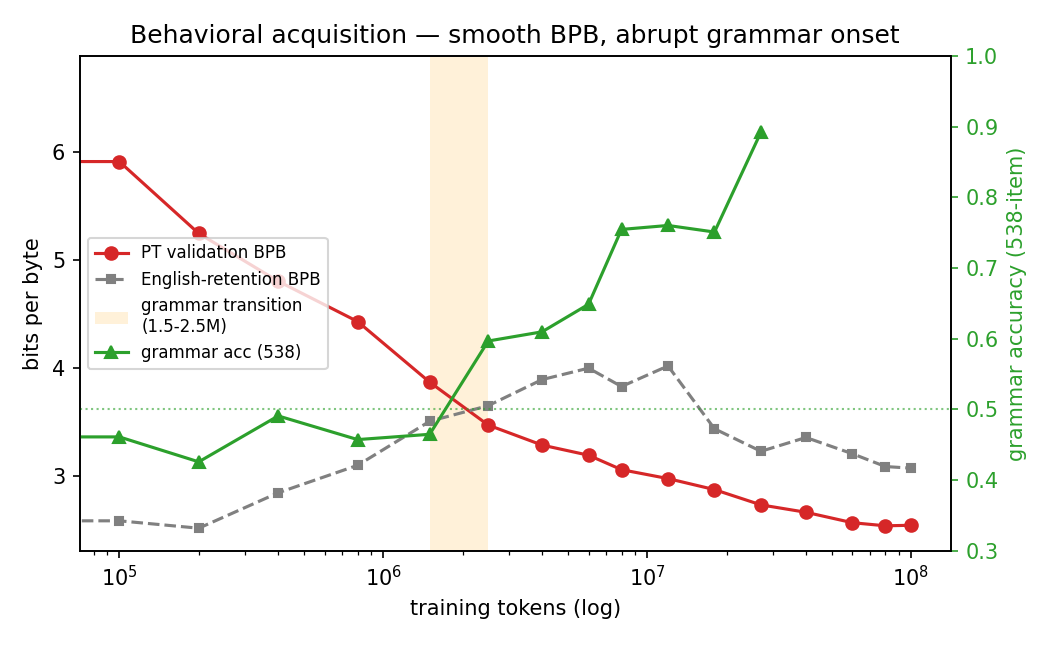
\includegraphics[width=0.82\textwidth]{figures/behavioral.png}
  \caption{Behavioral acquisition (structured PT, seed~A). PT BPB (red) falls
  smoothly; the 538-item grammar accuracy (green, right axis) is flat at chance
  then rises sharply through the shaded $1.5$--$2.5$M window. English-retention
  BPB (grey) degrades then partly recovers.}
  \label{fig:behavior}
\end{figure}

\begin{table}[H]
  \centering\small
  \begin{tabular}{rrrrr}
    \toprule
    tokens & PT BPB & EN BPB & grammar acc. & grammar margin\\
    \midrule
    0      & 6.686 & 2.714 & 0.446 & $-0.277$\\
    1.5M   & 3.869 & 3.506 & 0.465 & $-0.394$\\
    \textbf{2.5M} & 3.471 & 3.651 & \textbf{0.597} & $\mathbf{+0.461}$\\
    8M     & 3.057 & 3.829 & 0.755 & $+1.540$\\
    27M    & 2.731 & 3.228 & 0.892 & $+2.403$\\
    100M   & 2.541 & 3.071 & --- & ---\\
    \bottomrule
  \end{tabular}
  \caption{Behavioral trajectory (structured PT, seed~A). The grammar margin
  crosses zero at $\approx\!2.5$M tokens. Grammar was scored to $27$M (the
  transition is well before); BPB to $100$M.}
  \label{tab:behavior}
\end{table}

\subsection{The LLC trajectory: a rise-then-plateau changepoint}\label{sec:llc}
The LLC is positive at every checkpoint, with tight chain agreement and no
rejected chains. It rises $\approx\!34$ points over $400$k$\rightarrow$$4$M
(steepest through $400$k--$2.5$M) and is then flat within noise ($\approx\!84$--$87$)
for the remaining $25\times$ of training (Figure~\ref{fig:llc_align}, left;
Table~\ref{tab:llc}). The steep rise \emph{brackets} the behavioral grammar
transition: the geometry reorganizes through $\approx\!400$k--$2.5$M, the grammar
margin crosses zero at $\approx\!2.5$M, and both then settle
(Figure~\ref{fig:llc_align}, right). Read carefully, the LLC rise slightly
\emph{leads} the behavioral expression --- local complexity increases first,
grammatical behavior follows and continues maturing after $\lhat$ has plateaued.

\begin{table}[H]
  \centering\small
  \begin{tabular}{rrrrrrr}
    \toprule
    tokens & 400k & 800k & 1.5M & 2.5M & 8M & 100M\\
    \midrule
    $\lhat$ (seed~A) & $+52.3$ & $+61.5$ & $+75.5$ & $+80.7$ & $+86.0$ & $+86.7$\\
    \bottomrule
  \end{tabular}
  \caption{Primary LLC trajectory (structured PT, seed~A; loc $100$, 3 chains).
  Full 11-checkpoint trajectory in Figure~\ref{fig:llc_align}.}
  \label{tab:llc}
\end{table}

\begin{figure}[H]
  \centering
  \begin{subfigure}{0.49\textwidth}
    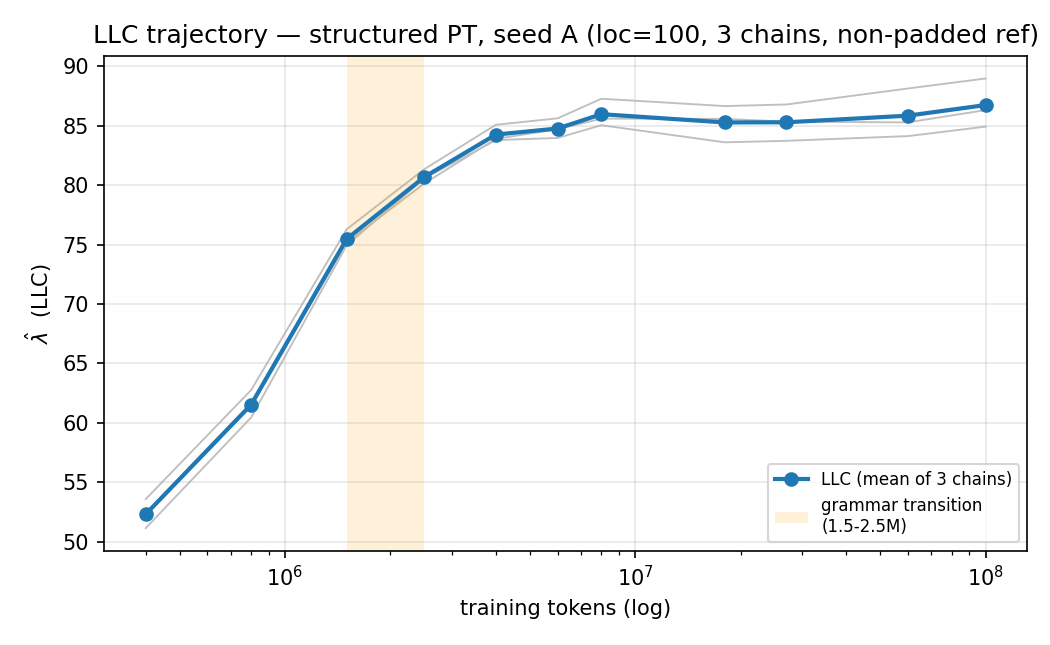
\includegraphics[width=\textwidth]{figures/llc_seedA.png}
  \end{subfigure}\hfill
  \begin{subfigure}{0.49\textwidth}
    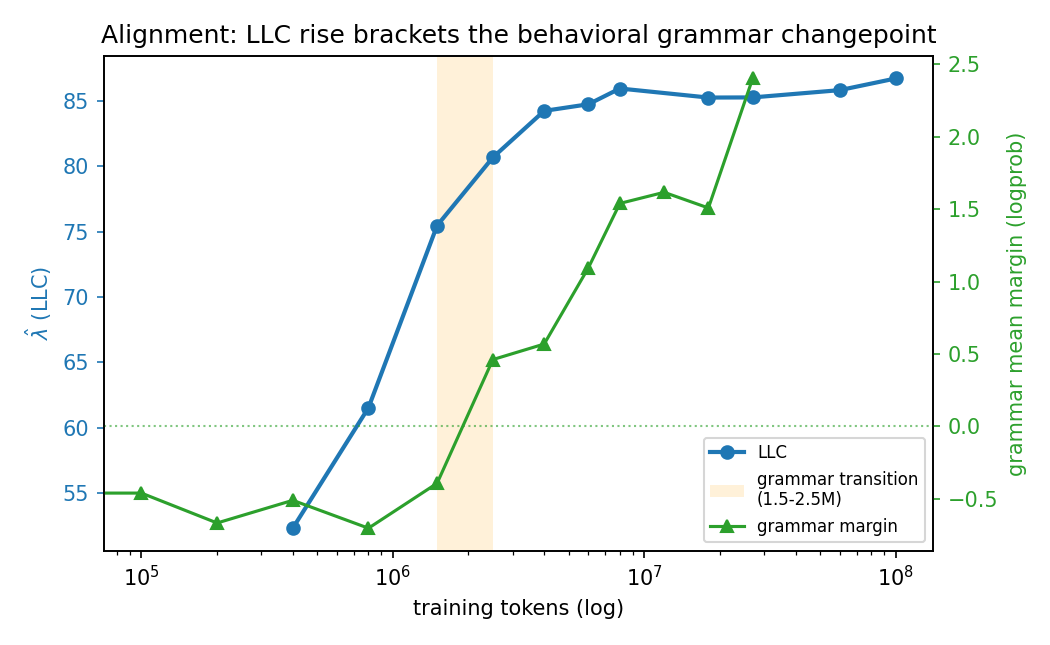
\includegraphics[width=\textwidth]{figures/alignment.png}
  \end{subfigure}
  \caption{\textbf{Left:} the LLC trajectory (structured PT, seed~A) rises
  steeply then plateaus; thin grey lines are individual chains. \textbf{Right:}
  alignment --- the LLC rise (blue) brackets the grammar-margin sign change
  (green) in the shaded $1.5$--$2.5$M window.}
  \label{fig:llc_align}
\end{figure}

\subsection{Controls: the changepoint is specific}\label{sec:controls}
Neither control reproduces the rise-then-plateau (Figure~\ref{fig:controls},
Table~\ref{tab:controls}). The token-shuffled model rises only weakly to
$\approx\!60$ and then \emph{declines} to $\approx\!28$ as it settles into
low-complexity position-independent statistics. The matched-English model
genuinely adapts (complexity rises monotonically $51\rightarrow70$) but
\emph{smoothly and to a markedly lower level}, with no steep transition and no
high plateau --- the key control showing the signature is not merely ``continued
pretraining raises the LLC.'' At $100$M the three conditions are cleanly
separated, and only structured Portuguese has both the steep grammar-window rise
and the high plateau. The geometric changepoint is therefore specific to genuine
Portuguese structure being acquired, not to training length, token statistics,
or generic adaptation.

\begin{table}[H]
  \centering\small
  \begin{tabular}{rrrr}
    \toprule
    tokens & structured PT & shuffled PT & matched EN\\
    \midrule
    1.5M  & $+75.5$ & $+60.4$ (peak) & $+58.8$\\
    8M    & $+86.0$ & $+43.2$ & $+64.8$\\
    100M  & $+86.7$ & $+27.9$ & $+70.3$\\
    \bottomrule
  \end{tabular}
  \caption{LLC at shared checkpoints across the three conditions (loc $100$,
  3 chains, condition-matched references).}
  \label{tab:controls}
\end{table}

\begin{figure}[H]
  \centering
  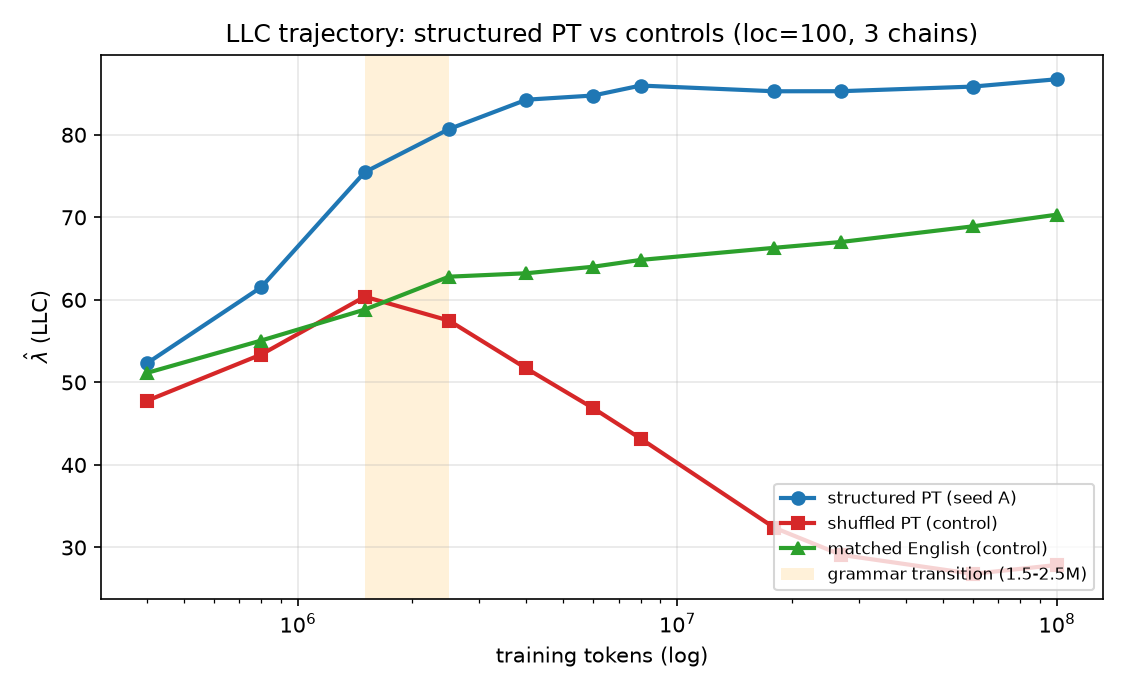
\includegraphics[width=0.82\textwidth]{figures/controls.png}
  \caption{Three-condition contrast. Structured PT (blue) rises to a high plateau;
  shuffled PT (red) rises then declines; matched English (green) rises smoothly to
  a lower level. The shaded band marks the behavioral grammar transition.}
  \label{fig:controls}
\end{figure}

\subsection{Robustness to the localization hyperparameter}\label{sec:robust}
The SGLD localization $\gamma$ sets the prior strength around the checkpoint, so
it shifts the absolute level of $\lhat$. At $\gamma=300$ the structured-PT
trajectory sits $\approx\!4$ units below $\gamma=100$ everywhere but is
\emph{identical in shape} --- same steep rise through $1.5$--$2.5$M, same plateau
(Figure~\ref{fig:loc}). The changepoint is thus a property of the trajectory, not
of the localization choice.

\begin{figure}[H]
  \centering
  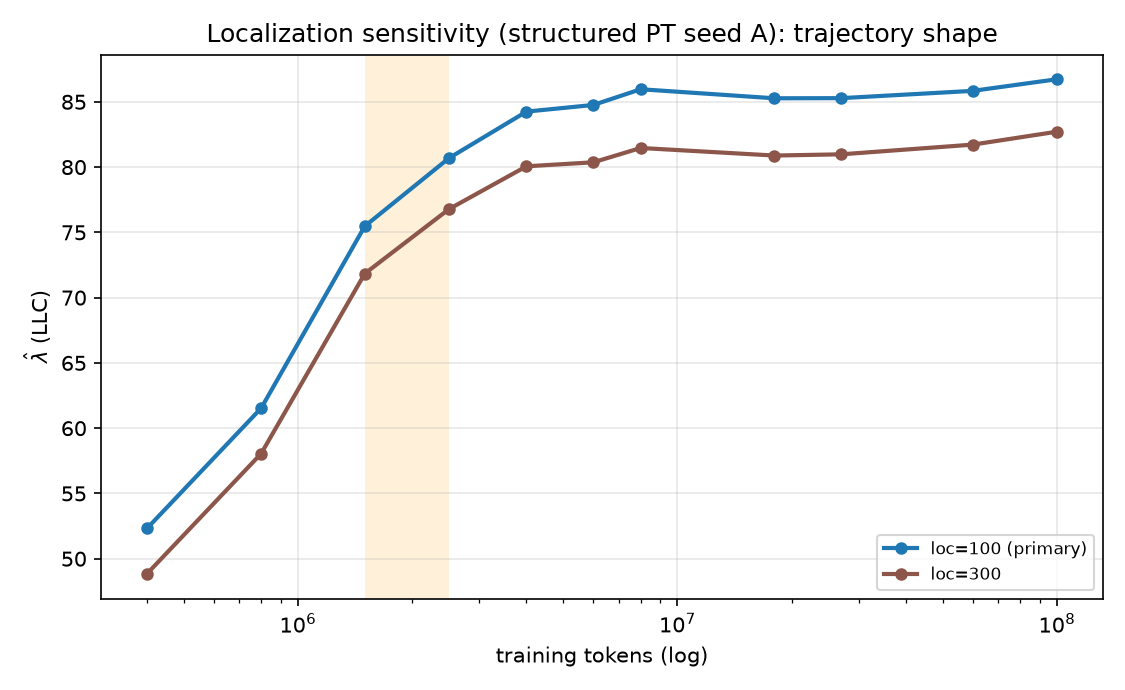
\includegraphics[width=0.72\textwidth]{figures/localization.png}
  \caption{Localization sensitivity (structured PT, seed~A): $\gamma=100$ vs.\
  $\gamma=300$ are near-parallel --- the rise-then-plateau shape is preserved.}
  \label{fig:loc}
\end{figure}

\section{Discussion}
Across an identical architecture, optimizer, and token budget, three conditions
produce three qualitatively different LLC trajectories, and only the one with
real grammatical structure to acquire shows a steep rise bracketing the moment
grammatical behavior appears. A geometric changepoint and a behavioral
changepoint coincide where the modeling-loss curve shows nothing. Following
standard caution we call this \emph{a changepoint in an SLT-derived local
geometric estimate aligned with a behavioral transition}, and we do not claim a
formal SLT phase transition, nor grokking (training and held-out performance
improve together). The slight \emph{lead} of the LLC over behavior is suggestive
of the geometry reorganizing before the capability is fully expressed, but we do
not over-read a single trajectory.

\section{Limitations}
\begin{itemize}\itemsep2pt
  \item \textbf{Single Portuguese seed.} The controls establish specificity but
  vary data \emph{content}, not the random seed; they do not rule out that the
  exact trajectory is idiosyncratic to one initialization / data order. A genuine
  second-seed replication (independent data ordering) is \emph{in progress} and
  will be folded in.
  \item \textbf{No formal changepoint test.} ``The rise brackets the transition''
  and ``the lead'' are read from the trajectories, not from a fitted changepoint
  model with a significance statement.
  \item \textbf{Localization sweep is two points} ($\gamma\in\{100,300\}$);
  shape-invariance over a wider range would strengthen the robustness claim.
  \item \textbf{Templated benchmark.} The 538-item grammar set is generated from
  agreement templates, not a validated broad-coverage suite.
\end{itemize}

\section{Conclusion}
In a small, fully controlled language-acquisition setting, an SLT-derived local
geometric quantity exhibits a changepoint aligned with the behavioral onset of
grammatical competence, shown specific by two controls and robust to the SGLD
localization. Pending a second-seed replication, this is, to our knowledge, a
clean demonstration of an LLC$\leftrightarrow$behavior alignment during
second-language acquisition.

% ---------------------------------------------------------------------------
% Indicative references --- VERIFY exact authors/titles/years before submission.
% ---------------------------------------------------------------------------
\begin{thebibliography}{9}
\bibitem{watanabe2009} S.~Watanabe.
  \emph{Algebraic Geometry and Statistical Learning Theory}.
  Cambridge University Press, 2009.
\bibitem{lau2024} E.~Lau, Z.~Furman, G.~Wei, D.~Murfet, S.~Wei.
  \emph{Quantifying degeneracy in singular models via the learning coefficient}.
  2023/2024 (devinterp).
\bibitem{hoogland2024} J.~Hoogland, G.~Wang, M.~Farrugia-Roberts, L.~Carroll,
  S.~Wei, D.~Murfet.
  \emph{The Developmental Landscape of In-Context Learning}. 2024.
\bibitem{chen2023} Z.~Chen et al.
  \emph{Dynamical versus Bayesian Phase Transitions in a Toy Model of
  Superposition}. 2023.
\end{thebibliography}

\end{document}
